\documentclass{standalone}

\usepackage{tikz}
\usepackage{standalone}
\usetikzlibrary{calc}
\usepackage{color}

\usetikzlibrary{decorations.pathmorphing}
\usetikzlibrary{fit}					% fitting shapes to coordinates
\usetikzlibrary{backgrounds}	% drawing the background after the foreground

\tikzstyle{background}=[red, rectangle, draw, inner sep=-1mm, dotted,
		   rounded corners=1mm]

\begin{document}

    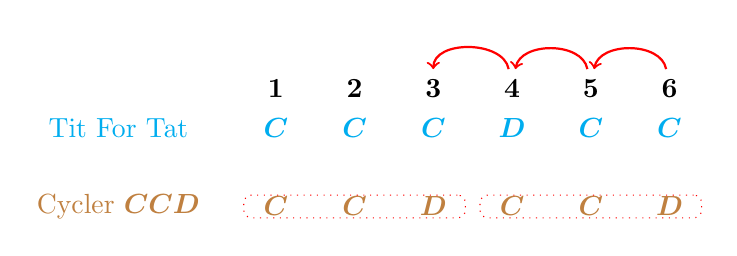
\begin{tikzpicture}

    \tikzstyle{state}=[minimum width=1cm, font=\boldmath];
    

	\node[thick] (0) at (-1, 0) [state] {\textcolor{cyan}{Tit For Tat}};
	\node[thick] (1) at (-1, -1) [state] {\textcolor{brown}{Cycler $CCD$}};

	\node[thick] (2) at (1, 0.5) [state] {$1$};
	\node[thick] (3) at (2, 0.5) [state] {$2$};
	\node[thick] (4) at (3, 0.5) [state] {$3$};
	\node[thick] (5) at (4, 0.5) [state] {$4$};
	\node[thick] (6) at (5, 0.5) [state] {$5$};
	\node[thick] (7) at (6, 0.5) [state] {$6$};

	\node (8) at (1, 0) [state] {\textcolor{cyan}{$C$}};
	\node (9) at (2, 0) [state] {\textcolor{cyan}{$C$}};
	\node (10) at (3, 0) [state] {\textcolor{cyan}{$C$}};
	\node (11) at (4, 0) [state] {\textcolor{cyan}{$D$}};
	\node (12) at (5, 0) [state] {\textcolor{cyan}{$C$}};
	\node (13) at (6, 0) [state] {\textcolor{cyan}{$C$}};

	\node (14) at (1, -1) [state] {\textcolor{brown}{$C$}};
	\node (15) at (2, -1) [state] {\textcolor{brown}{$C$}};
	\node (16) at (3, -1) [state] {\textcolor{brown}{$D$}};
	\node (17) at (4, -1) [state] {\textcolor{brown}{$C$}};
	\node (18) at (5, -1) [state] {\textcolor{brown}{$C$}};
	\node (19) at (6, -1) [state] {\textcolor{brown}{$D$}};

	\draw (5) edge[red, out=100, in=90, ->, thick] node [above] {} (4);
	\draw (6) edge[red, out=100, in=80, ->, thick] node [above] {} (5);
	\draw (7) edge[red, out=100, in=80, ->, thick] node [above] {} (6);

	\node [background, fit=(14) (15) (16)] {};
	\node [background, fit=(17) (18) (19)] {};

    \end{tikzpicture}

\end{document}